\chapter{Methods}
%The method chapter of this paper describes the process from creating a data capture pipeline, extending it to a full end-to-end capture-to-render pipeline with Nerfstudio, using the pipeline to create a data capture baseline, using the baseline to run further experiments, extending the baseline to support large scale scenes, and finally extending it to support real data.

This chapter is split into multiple parts, all essential for the end-to-end pipeline, depicted in \autoref{fig:end-to-end-pipeline}, to allow the capture of data and subsequent training, evaluation, and render of a NeRF with Nerfstudio. The separate components are thoroughly explained.

% TODO: Write that we're going to use Nerfstudio here?

\begin{figure}[ht]
    \centering
    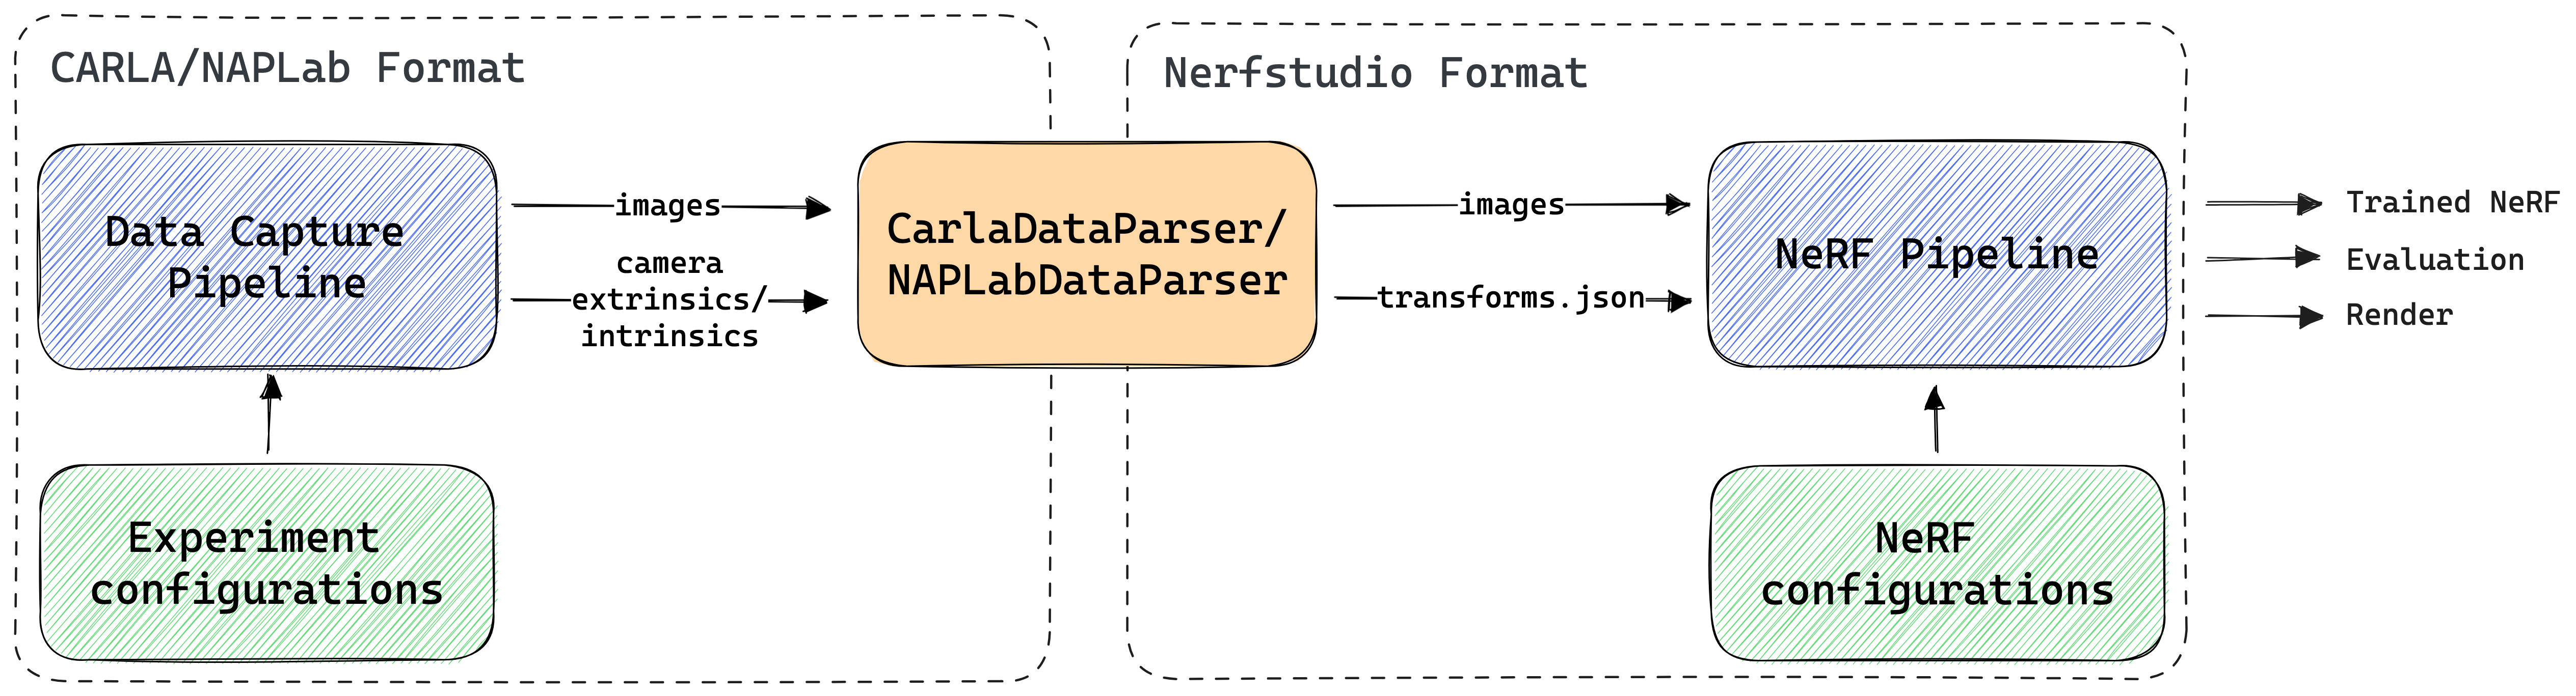
\includegraphics[width=1.0\textwidth]{figures/end-to-end-pipeline-v2.png}
    \caption[Overview of the end-to-end pipeline.]{Overview of the end-to-end pipeline that captures data from CARLA or the \acrshort{naplab} car, converts the data into Nerfstudio format, and utilizes the resulting data to train, evaluate, and render a camera path for the NeRF.}
    \label{fig:end-to-end-pipeline}
\end{figure}

\begin{comment}
This chapter elucidates the methodological approach employed in this research to explore the potential of Neural Radiance Fields (NeRF) in improving the synthetic data pipeline from CARLA to Nerfstudio. Our approach is underpinned by a systematic series of stages, each contributing to the robustness of the pipeline, and enabling us to establish a baseline leveraging synthetic data from CARLA.

We start this chapter by detailing the process of collecting synthetic data from CARLA, a sophisticated platform for generating artificial datasets. We explain our selection criteria and data collection techniques, aimed at maintaining consistency while ensuring the collected data is representative and fit for our objectives.

Next, we outline our procedure for integrating the collected data into the Nerfstudio environment. Our goal here is to ensure seamless data transition, optimising the pipeline for robust performance. A detailed description of the specific pipeline we created with CARLA data in Nerfstudio will follow.

A significant component of our method is establishing a CARLA baseline. We elucidate how this baseline was identified and what parameters were considered. Following the establishment of the baseline, we detail its application in various stages of our method.

The subsequent section focuses on the extension of the CARLA-baseline to support large-scale scenes using the concept of Block-NeRF. This is a vital aspect of our method that enables more extensive and complex scene rendering, thus broadening the application scope of our pipeline.

Lastly, we present an extension of the pipeline to accommodate input of real data, providing a pathway for future integration of real-world scenarios into the existing synthetic data pipeline. This element of our method is critical in considering the practicability of our pipeline beyond synthetic data environments.

By sequentially guiding the reader through our method, this chapter seeks to offer comprehensive insight into our research approach, underlying decisions, and considerations. This will lay a strong foundation for understanding the experimental results and discussions in the subsequent chapters.
\end{comment}

%\section{Data capture pipeline - Collect synthetic data from CARLA}
\section{Implementing the CARLA Data Capture Pipeline}
This section will explain how we utilize the CARLA-simulator, introduced in \autoref{sec:carla}, to capture synthetic data. It'll cover basic CARLA-concepts and give a thorough explanation of how the different concepts are combined and utilized in order to create a data capture pipeline.

\begin{comment}

Premise: Have no data to train a NeRF on
Question: How can we collect synthetic data from CARLA?

\begin{itemize}
    \item How can you spawn an agent, etc?
    \item How does all the basic CARLA-things work? 
    \item How to mount cameras, which sensors, location and rotation (transform).
\end{itemize}
\end{comment}

\begin{comment}
    
% Code: generic_nerf_capture.py
\subsubsection{Connecting the CARLA API to a CARLA simulator}
I might add something here about how the data flows in the CARLA setup.

In order to run experiments 
\end{comment}



\subsubsection{Creating a CARLA Actor}
To capture data in the virtual CARLA-environment, a vehicle that is both controllable and programmable is required. This vehicle is commonly referred to as the “ego” vehicle (\texttt{carla.Vehicle}) and is a special instance of the most basic CARLA instance, the \texttt{carla.Actor}. It can be spawned by defining a spawn point, a choice of vehicle, and whether the vehicle should operate on autopilot or not. Although an arbitrary number of autopilot vehicles can be spawned to simulate a complex traffic environment, the objective is to capture synthetic data with minimal transient objects; therefore, only the ego vehicle is spawned.


\subsubsection{Setting up the environment with the traffic manager}

In order to define the environment in which the spawned ego vehicle will operate, we leverage the \texttt{carla.TrafficManager} available on the \texttt{carla.Client} that's used to connect to the simulator. The traffic manager enables us to define some important aspects of the environment:

\begin{itemize}
    \item \textbf{Choose the ego vehicle's route:} The traffic manager allows us to set the route instructions for a specific actor. We can define arbitrary routes by creating an array of route instructions, e.g. \texttt{['Left', 'Left', 'Right', 'Straight', 'Right']}.
    \item \textbf{Choose to ignore the traffic lights:} Since the only moving vehicle in the environment is the ego vehicle, we don't have to abide by the rules of traffic. In order to speed up the data capture we choose to ignore the traffic lights.
    \item \textbf{Set the vehicle speed:} The traffic manager provides the ability to configure a vehicle’s speed as a percentage of the default speed of 30 km/h. A setting of $100\%$ adheres to the default speed, while a setting of $50\%$ corresponds to a speed of 15 km/h, and so on.
\end{itemize}


\subsubsection{Experiment configuration}
In order to evaluate numerous environment and vehicle setups, along with their corresponding outcomes, an \texttt{ExperimentConfig}-class was created. This class enables the definition of the following configurations:

\begin{itemize}
    \item \textbf{Camera rig:} Mounts a list of RGB-cameras with configurable camera settings, location, and rotation to the ego vehicle. We're optionally able to parse a "rig"-file, a special type of JSON file exported from the NAPLab car discussed in \autoref{sec:extending-real-data}, into a camera rig for the ego vehicle. 
    \item \textbf{Data capture frequency}: Sets the frequency of data capture, i.e. images and camera poses.
    \item \textbf{Stop-criteria:} Specifies the ego vehicle's stop condition either by a stop distance or a number of completed turns.
    \item \textbf{Camera noise:} Enables the simulation of noisy GPS/GNSS sensor readings by adding Gaussian noise to the location output from the mounted cameras.
    \item \textbf{Spawn transform:} Enables specifying the spawn-location/-rotation of the ego vehicle.
    \item \textbf{Speed:} Sets the target speed for the ego vehicle.
    \item \textbf{Route:} Sets the route instructions for the ego vehicle.
\end{itemize}


\subsubsection{CARLA data parser}

To capture and store data during the vehicle’s drive, a custom \texttt{CarlaDataParser}-class is created. This class provides methods for capturing an image with its corresponding camera pose, transforming the camera poses into specified formats, and exporting the captured data. The format and data conventions will be thoroughly described in \autoref{sec:carla-to-nerfstudio}.

\subsubsection{CARLA Run-loop}
The CARLA Run-loop includes the following steps:

\begin{itemize}
    \item Read and apply the configurations from \texttt{ExperimentConfig}.
    \item Spawn an ego vehicle.
    \item While the ego vehicle hasn’t met a stop-criteria, e.g. that it has driven the set amount of distance/turns, keep driving and capture data.
    \begin{itemize}
        \item Get the image from all the cameras mounted to the car: Each sensor in CARLA has a \texttt{listen} method, triggered whenever data is retrieved by the sensor. The Carlo-repository\footnote{\url{https://github.com/aasewold/carlo/}} simplifies the process of obtaining image data from the corresponding camera, a process which traditionally would involve managing the listen-callback, decoding the \texttt{carla.Image} data, and converting raw data bytes into \texttt{np.ndarrays}. Using the Carlo abstraction, the steps are reduced to creating a list of cameras, retrieving the \texttt{np.ndarray} containing the image data, stacking the camera outputs, and presenting the resulting image using a library like \texttt{OpenCV} \cite{opencv_library}.
        \item Pass the captured image and corresponding camera pose to the \texttt{CarlaDataParser}'s \texttt{append\_frame} method.
    \end{itemize}
    \item Export the parsed CARLA-data with \texttt{CarlaDataParser}'s \texttt{export\_transforms} method.
    \item Terminate the simulation and perform necessary clean-up activities.
\end{itemize}


\begin{comment}
The following algorithm outlines the steps for capturing synthetic data using the CARLA simulator. The code is written in Python and utilizes the CARLA library.

    
\begin{algorithmic}[1]
\Function{run\_carla\_session}{experiment\_settings}
    \State \textbf{create a directory} for the experiment and save experiment settings to a file
    \State \textbf{create a SLURM script} for the experiment
    \State \textbf{spawn an ego vehicle} and set up the traffic manager
    \State \textbf{create cameras} based on the specified camera rigs and rig file
    \State \textbf{create a TransformFile} to store the image and camera pose data
    \While{\textbf{stop criteria has not been met}}
        \State \textbf{tick the CARLA world}
        \State \textbf{get images} from all mounted cameras and stack them horizontally
        \State \textbf{show the image}
        \State \textbf{store the image and camera pose data} every n-th tick
        \State \textbf{update the distance traveled} using euclidean distance
    \EndWhile
    \State \textbf{export the TransformFile} and destroy the actors
\EndFunction
\end{algorithmic}

\end{comment}











%\section{CARLA Data Parser - From CARLA to Nerfstudio} \label{sec:carla-to-nerfstudio}
\section{Implementing the CARLA Data Parser for Nerfstudio} \label{sec:carla-to-nerfstudio}
\begin{comment}
Premise: Have collected data from CARLA.
Question: How do I get it from CARLA to Nerfstudio in a usable format?

\begin{itemize}
    \item Use the CARLA-simulator to find out which camera and vehicle settings work the best for capturing data for NeRFs.
    \item In order to do that I need to collect data from CARLA and convert it into a format that's usable by Nerfstudio.
\end{itemize}
\end{comment}

Having obtained a pipeline that enables the creation of a controllable environment for a vehicle with an arbitrary setup of sensors, and subsequent data-capture, the captured data have to be exported in a format readable by Nefstudio. This section will elaborate on the creation of \texttt{CarlaDataParser} and the conversion from CARLA to Nerfstudio

% We now have a pipeline that enables the creation of a controllable environment for a vehicle with an arbitrary setup of sensors, and subsequent capture of data. How do we export the captured sensor data in a format that's readable by Nerfstudio?

In order to train a NeRF we need images and corresponding camera poses. As discussed in \autoref{sec:nerf}, the camera poses are $4x4$ homogeneous transformation matrices, containing both the translation and rotation in reference to a coordinate system. Nerfstudio, as discussed in \autoref{sec:nerfstudio}, expects the data in a file structure as shown in \autoref{fig:nerfstudio-file-structure}. In order to handle the data parsing from CARLA to Nerfstudio we create a helper-class \texttt{CarlaDataParser} which has methods for saving images as PNG files, calculating the camera's intrinsic parameters, transforming the extrinsic parameters, and appending parsed frames to a \texttt{transforms.json}-file. The \texttt{transforms.json}-file contains the camera's intrinsics and a list of frames where each frame holds an image path and the respective image's camera pose. An example \texttt{transforms.json}-file can be seen in \autoref{code:transform-examples}.

\begin{figure}[ht]
\centering
\begin{forest}
for tree={
      parent anchor=south west,
      child anchor=west,
      anchor=mid west,
      inner ysep=1pt,
      grow'=0,
      align=left,
      edge path={
        \noexpand\path [draw, \forestoption{edge}] (!u.parent anchor) ++(1em,0) |- (.child anchor)\forestoption{edge label};
      },
      font=\sffamily,
      if n children=0{}{
        delay={
          prepend={[,phantom, calign with current]}
        }
      },
      fit=band,
      before computing xy={
        l=2em
      }
    }
[ your\_nerf\_data/
  [ images/
    [ 0001.png ]
    [ 0002.png ]
    [ 0003.png ]
    [ \ldots{} ]
  ]
  [ transforms.json ]
]
\end{forest}
\caption{File structure expected by Nerfstudio}
\label{fig:nerfstudio-file-structure}
\end{figure}
\begin{figure}[ht]
\centering
\begin{lstlisting}[language=json,linewidth=0.9\linewidth]
{
    "camera_model": "OPENCV",
    "fl_x": 200.0,
    "fl_y": 150.0,
    "cx": 200.0,
    "cy": 150.0,
    "w": 400,
    "h": 300,
    "k1": 0,
    "k2": 0,
    "p1": 0,
    "p2": 0,
    "frames": [...]
}
\end{lstlisting}
\caption{Example of a \texttt{transforms.json}-file with the intrinsic parameters and a collapsed list of frames containing the extrinsic parameters of the camera.}
\label{code:transform-examples}
\end{figure}


CARLA gives access to basic camera attributes that we can use to approximate the intrinsic parameters. Given the image's width $w$ and height $h$, in accordance to the camera's \acrfull{fov}, we can calculate the focal length $f$ and subsequently the $x$- and $y$-component of the focal length $f_x$ and $f_y$ as follows:

\begin{align*}
f &= \tan\left(\frac{\text{FOV}}{2}\right) &
f_x &= \frac{0.5 \times w}{f} &
f_y &= \frac{0.5 \times h}{f}
\end{align*}

The camera's principal points $c_x$ and $c_y$ are assumed to be the center of the image plane, and obtained with:

\begin{align*}
c_x &= \frac{w}{2} &
c_y &= \frac{h}{2}
\end{align*}

Once calculated, the intrinsic values are added to the \texttt{transforms.json}-file.

CARLA is built with Unreal Engine and subsequently uses its coordinate convention. The Unreal Engine coordinate convention, illustrated in \autoref{fig:carla-coordinates-system}, is a left-handed system where +X is forward, +Y is right, and +Z is up. Nerfstudio uses the OpenGL/Blender coordinate convention for cameras, which is a right-handed system, and its world space is oriented such that +X is right, +Y is forward, and +Z is up. The disparity in coordinate conventions between CARLA and Nerfstudio would make the NeRF-renderings non-interpretable, if we trained a NeRF directly on the transformation matrices exported from CARLA. In order to convert the transformation matrices that contain both rotation and translation we apply \texttt{CarlaDataParser}'s \texttt{carla\_to\_nerf}-transformation. The transformation from CARLA's left-handed coordinate system to NerfStudio's right-handed coordinate system can be represented as a matrix multiplication.

Let $M_{carla}$ be the transformation matrix in CARLA convention, and $M_{nerf}$ be the transformation matrix in Nerfstudio convention. The transformation can be expressed as:

$$M_{nerf} = R_{z}(90) \cdot R_{x}(-90) \cdot T \cdot M_{carla} $$

where $T$ is a translation matrix to swap the y and z coordinates, and $R_{x}$, $R_{z}$ are rotation matrices around the x and z axes, respectively. The order of multiplication is from right to left.

% ------
\begin{comment}
    
as described in \textbf{INSERT FIGURE/EQUATION HERE}, before appending the frame to the \texttt{transforms.json}-file. The \texttt{carla\_to\_nerf} function takes a \texttt{carla.Transform} object as input and returns a 4x4 matrix in OpenGL/Blender-format. The function first extracts the location and rotation components of the input transform. The location component is then converted from the Unreal Engine coordinate system to the OpenGL/Blender coordinate system used by Nerfstudio. This conversion involves swapping the X and Y coordinates of the location and negating the Z coordinate. The rotation component is also converted to the OpenGL/Blender coordinate system by swapping the pitch and roll angles and adding 90 degrees to each angle. Finally, the transformed location and rotation components are combined into a new \texttt{carla.Transform} object, which is used to generate the 4x4 matrix that is returned by the function. An example of the transformed CARLA-matrix can be seen in \autoref{code:frame-example}.

\end{comment}
% ----------------------------------------















%\section{Nerfstudio pipeline with CARLA-data} \label{sec:nerfstudio-pipeline}
\section{Implementing the NeRF Pipeline} \label{sec:nerfstudio-pipeline}
\begin{comment}
Premise: Have data in a Nerfstudio format, collected from CARLA.
Question: How can I train a NeRF that represent the same scene?

\begin{itemize}
    \item Explain the Nerfstudio API and the created pipeline. Train, eval, render
    \item Go into detail on e.g. the train/eval-split, training parameters, etc. Add additional info to the appendix.
\end{itemize}
\end{comment}



%We now have the synthetic data captured from CARLA in a format that we can use to train NeRFs in Nerfstudio on. How do I use this data and the Nerfstudio API to create a pipeline that automates processing, training, evaluating and rendering the different experiments?

%I've created a pipeline that leverage the Nerfstudio API to process, train, evaluate, and render the NeRFs. The pipeline accepts parameters including:

Having obtained the synthetic data captured from CARLA in a format suitable for training NeRFs in Nerfstudio, the next step is to develop and utilize a pipeline that automates the processing, training, evaluation, and rendering of various experiments using this data and the Nerfstudio API. This section will elaborate on the pipeline and its components depicted in \autoref{fig:nerfstudio-pipeline}.

\begin{figure}[!h]
    \centering
    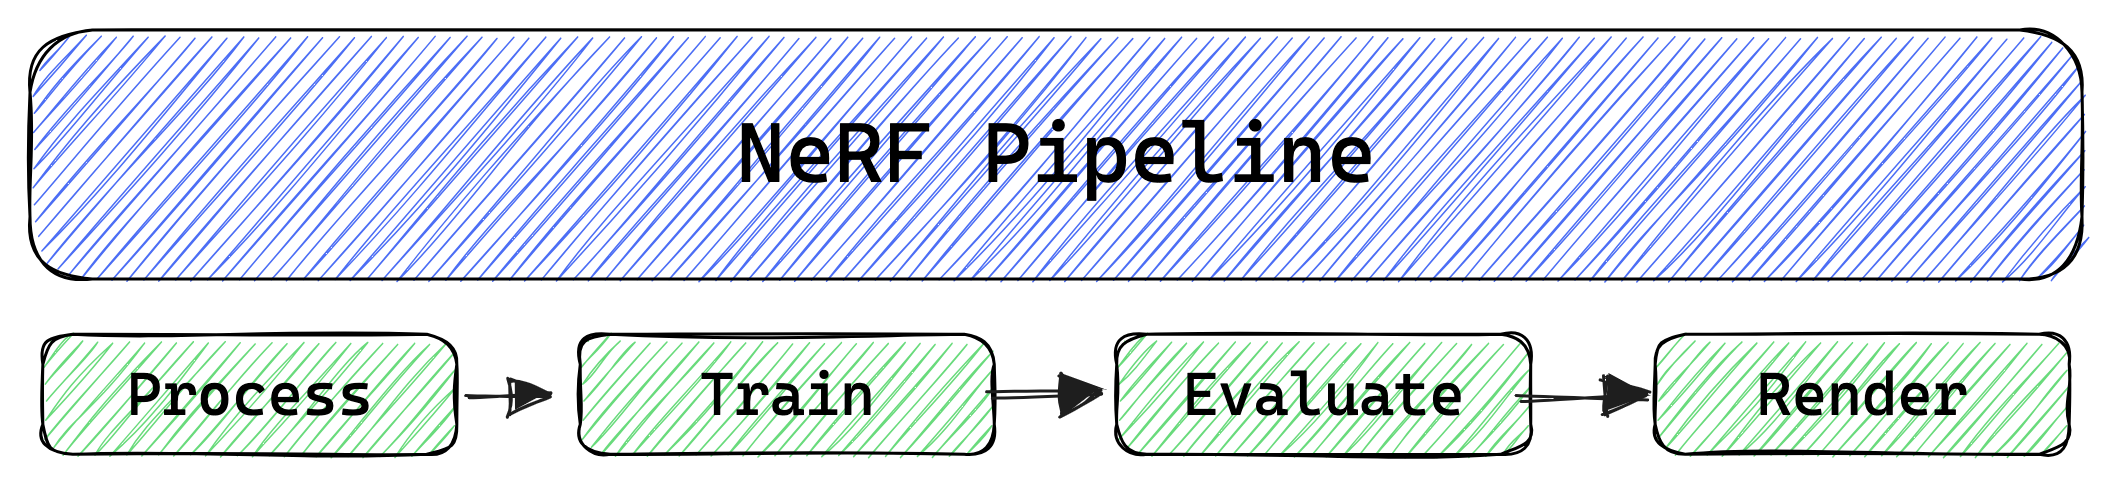
\includegraphics[width=1.0\textwidth]{figures/nerfstudio-pipeline.png}
    \caption{The components of the NeRF pipeline implemented in Nerfstudio.}
    \label{fig:nerfstudio-pipeline}
\end{figure}

The developed pipeline accepts a \texttt{Argument}-class used to configure the processing, training, evaluation, and rendering of the NerF. The most important parameters include:

\begin{itemize}
    \item \textbf{Input/output directory:} Defines where the data is located and where the output from the pipeline should be stored?
    \item \textbf{Model:} Defines which NeRF-model to use.
    \item \textbf{Settings for camera optimizer:} Defines if the NeRF should treat the camera poses as learnable parameters and optimize the camera poses.
    \item \textbf{Settings for side-by-side rendering:} Defines, among other things, which input-camera should be used as ground truth when rendering side-by-side.
\end{itemize}

\subsubsection{Process}

In most scenarios when working with real data, e.g. images of an object captured with a handheld camera, we don't have accurate camera poses. In those scenarios we have to pre-process the data in order to approximate camera poses for the captured images. It can be accomplished by leveraging SfM-algorithms as discussed in \autoref{sec:colmap}. In the scenario where the data is captured from CARLA, the poses are as accurate as they can be as they've been calculated in a deterministic environment. Assuming the CARLA-data is parsed according to the method discussed in \autoref{sec:carla-to-nerfstudio}, no further preprocessing is necessary.

\subsubsection{Train}
During training, the parameters in the model are optimized to represent the 3D scene. A batch of pixels is created for each training iteration. The default batch of 4096 pixels is obtained by randomly sampling the training images which defaults to $90\%$ of the total dataset, leaving $10\%$ as an evaluation dataset. Rays are marched through the sampled pixels and the model's networks predict RGB values and densities for the points sampled along the rays. The points' values are composited and the photometric loss, in combination with more complex losses, is computed. The losses are backpropagated through the model's networks and the ADAM optimizer\cite{adam} is used to update the network parameters.

For the Nerfacto-model, the primary model used throughout this thesis and previously discussed in \autoref{sec:nerfacto}, the training process entails backpropagating the loss and updating both the NeRF MLP and the proposal MLP. The Nerfacto-model leverages three different losses to guide the training; \textit{photometric loss}, \textit{interlevel loss}, and \textit{distortion loss}. \textit{Photometric loss} is the standard NeRF-loss explained in \autoref{eq:nerf-loss}. Interlevel- and distortion-loss are both from the Mip-NeRF 360\cite{barron_mip-nerf_2022} implementation explained in \autoref{sec:mipnerf360}. The interlevel loss encourages the model to generate consistent predictions across different levels of the multi-scale hierarchy, while the distortion loss encourages the model to generate smooth and continuous predictions.

Nerfstudio provides an API to configure all aspects of the pipeline, including dataset-split, number of pixels to sample, which optimizer to use, the configuration of the optimizer's exponential decay, the neural network's dimensionality, and much more. The implementation details and configurations used for the models in this thesis are attached in \autoref{sec:nerfstudio-train-parameters}.



\begin{comment}
The experiments in this thesis focus on the faster NeRF models implemented in Nerfstudio, namely Nerfacto (\autoref{sec:nerfacto}) and Instant NGP (\autoref{sec:instant-ngp}). Although the models are different, most of the shared model configurations are the same as can be seen in the model parameters included in \autoref{sec:nerfstudio-train-parameters}.

During training, the parameters in the model are trained to represent the 3D scene. For the Nerfacto-model, this entails backpropagating the error and updating both the NeRF MLP and the proposal MLP. The Nerfacto- and Instant NGP-model leverage 3 different losses to guide the training; \textit{RGB loss}, \textit{interlevel loss} and \textit{distortion loss}. \textit{RGB loss} is the standard NeRF-loss explained in \autoref{eq:nerf-loss}. Interlevel- and distortion-loss are both from the Mip-NeRF 360 implementation explained in \autoref{sec:mipnerf360}. The interlevel loss encourages the model to generate consistent predictions across different levels of the multi-scale hierarchy, while the distortion loss encourages the model to generate smooth and continuous predictions.

The training leverages the ADAM optimizer \cite{adam} for all networks within the model. The optimizer for the proposal networks and Nerfacto fields both use a learning rate of $1 \times 10^{-2}$, with no weight decay and $\epsilon=10^{-8}$, while the camera optimizer uses a learning rate of $6 \times 10^{-4}$, weight decay of $1 \times 10^{-2}$, and $\epsilon=10^{-8}$. All scenes were trained for 15,000 iterations, which is sufficient for achieving convergence. Training time for each scene is approximately 15-20 minutes when using an NVIDIA A100 GPU.

% TODO: Rewrite and reorganize. Write about how a batch of pixels are created for each training iteration
During the training of a NeRF, a batch of pixels is created for each training iteration. By default, this batch consists of 4096 pixels. To obtain these pixels, the training algorithm randomly samples them from all of the training images that are stored in RAM. However, this approach can be memory-intensive, especially when dealing with large datasets. To address this issue, the NeRF pipeline provides an option to set the parameter \texttt{–-pipeline.datamanager.train-num-images-to-sample-from}, which allows the user to sample pixels from a smaller subset of images. When using a smaller subset of images, the training algorithm will keep sampling from this subset unless the parameter \texttt{--num-times-to-repeat-images} is also set. This parameter specifies the number of training iterations after which the training algorithm should grab a new set of images to sample from. For instance, if \texttt{--num-times-to-repeat-images} is set to 1, the training algorithm will grab a new set of images to sample from every iteration. However, this approach can be computationally expensive and slow down the training process.
\end{comment}




\subsubsection{Evaluate}
To quantitatively evaluate the quality of the NeRF models, we utilize the metrics PSNR, SSIM, and LPIPS, as elaborated upon in \autoref{sec:evaluating-nerfs}. During the evaluation, the camera poses from the evaluation dataset are fed into the trained model which subsequently renders the novel views. The rendered images are then compared against the corresponding ground truth images from the evaluation dataset according to the aforementioned metrics. 

The Nerfstudio API provides a script to load a model-checkpoint and compute these metrics, providing a quantitative assessment of the trained NeRF. To further facilitate the comparison of NeRF models across multiple experiments, an additional script was developed. This script load the evaluation outputs, compares the resulting metrics and produces a formatted LaTeX table that highlights the best and worst metrics.

%\begin{figure}[h]
    \centering
    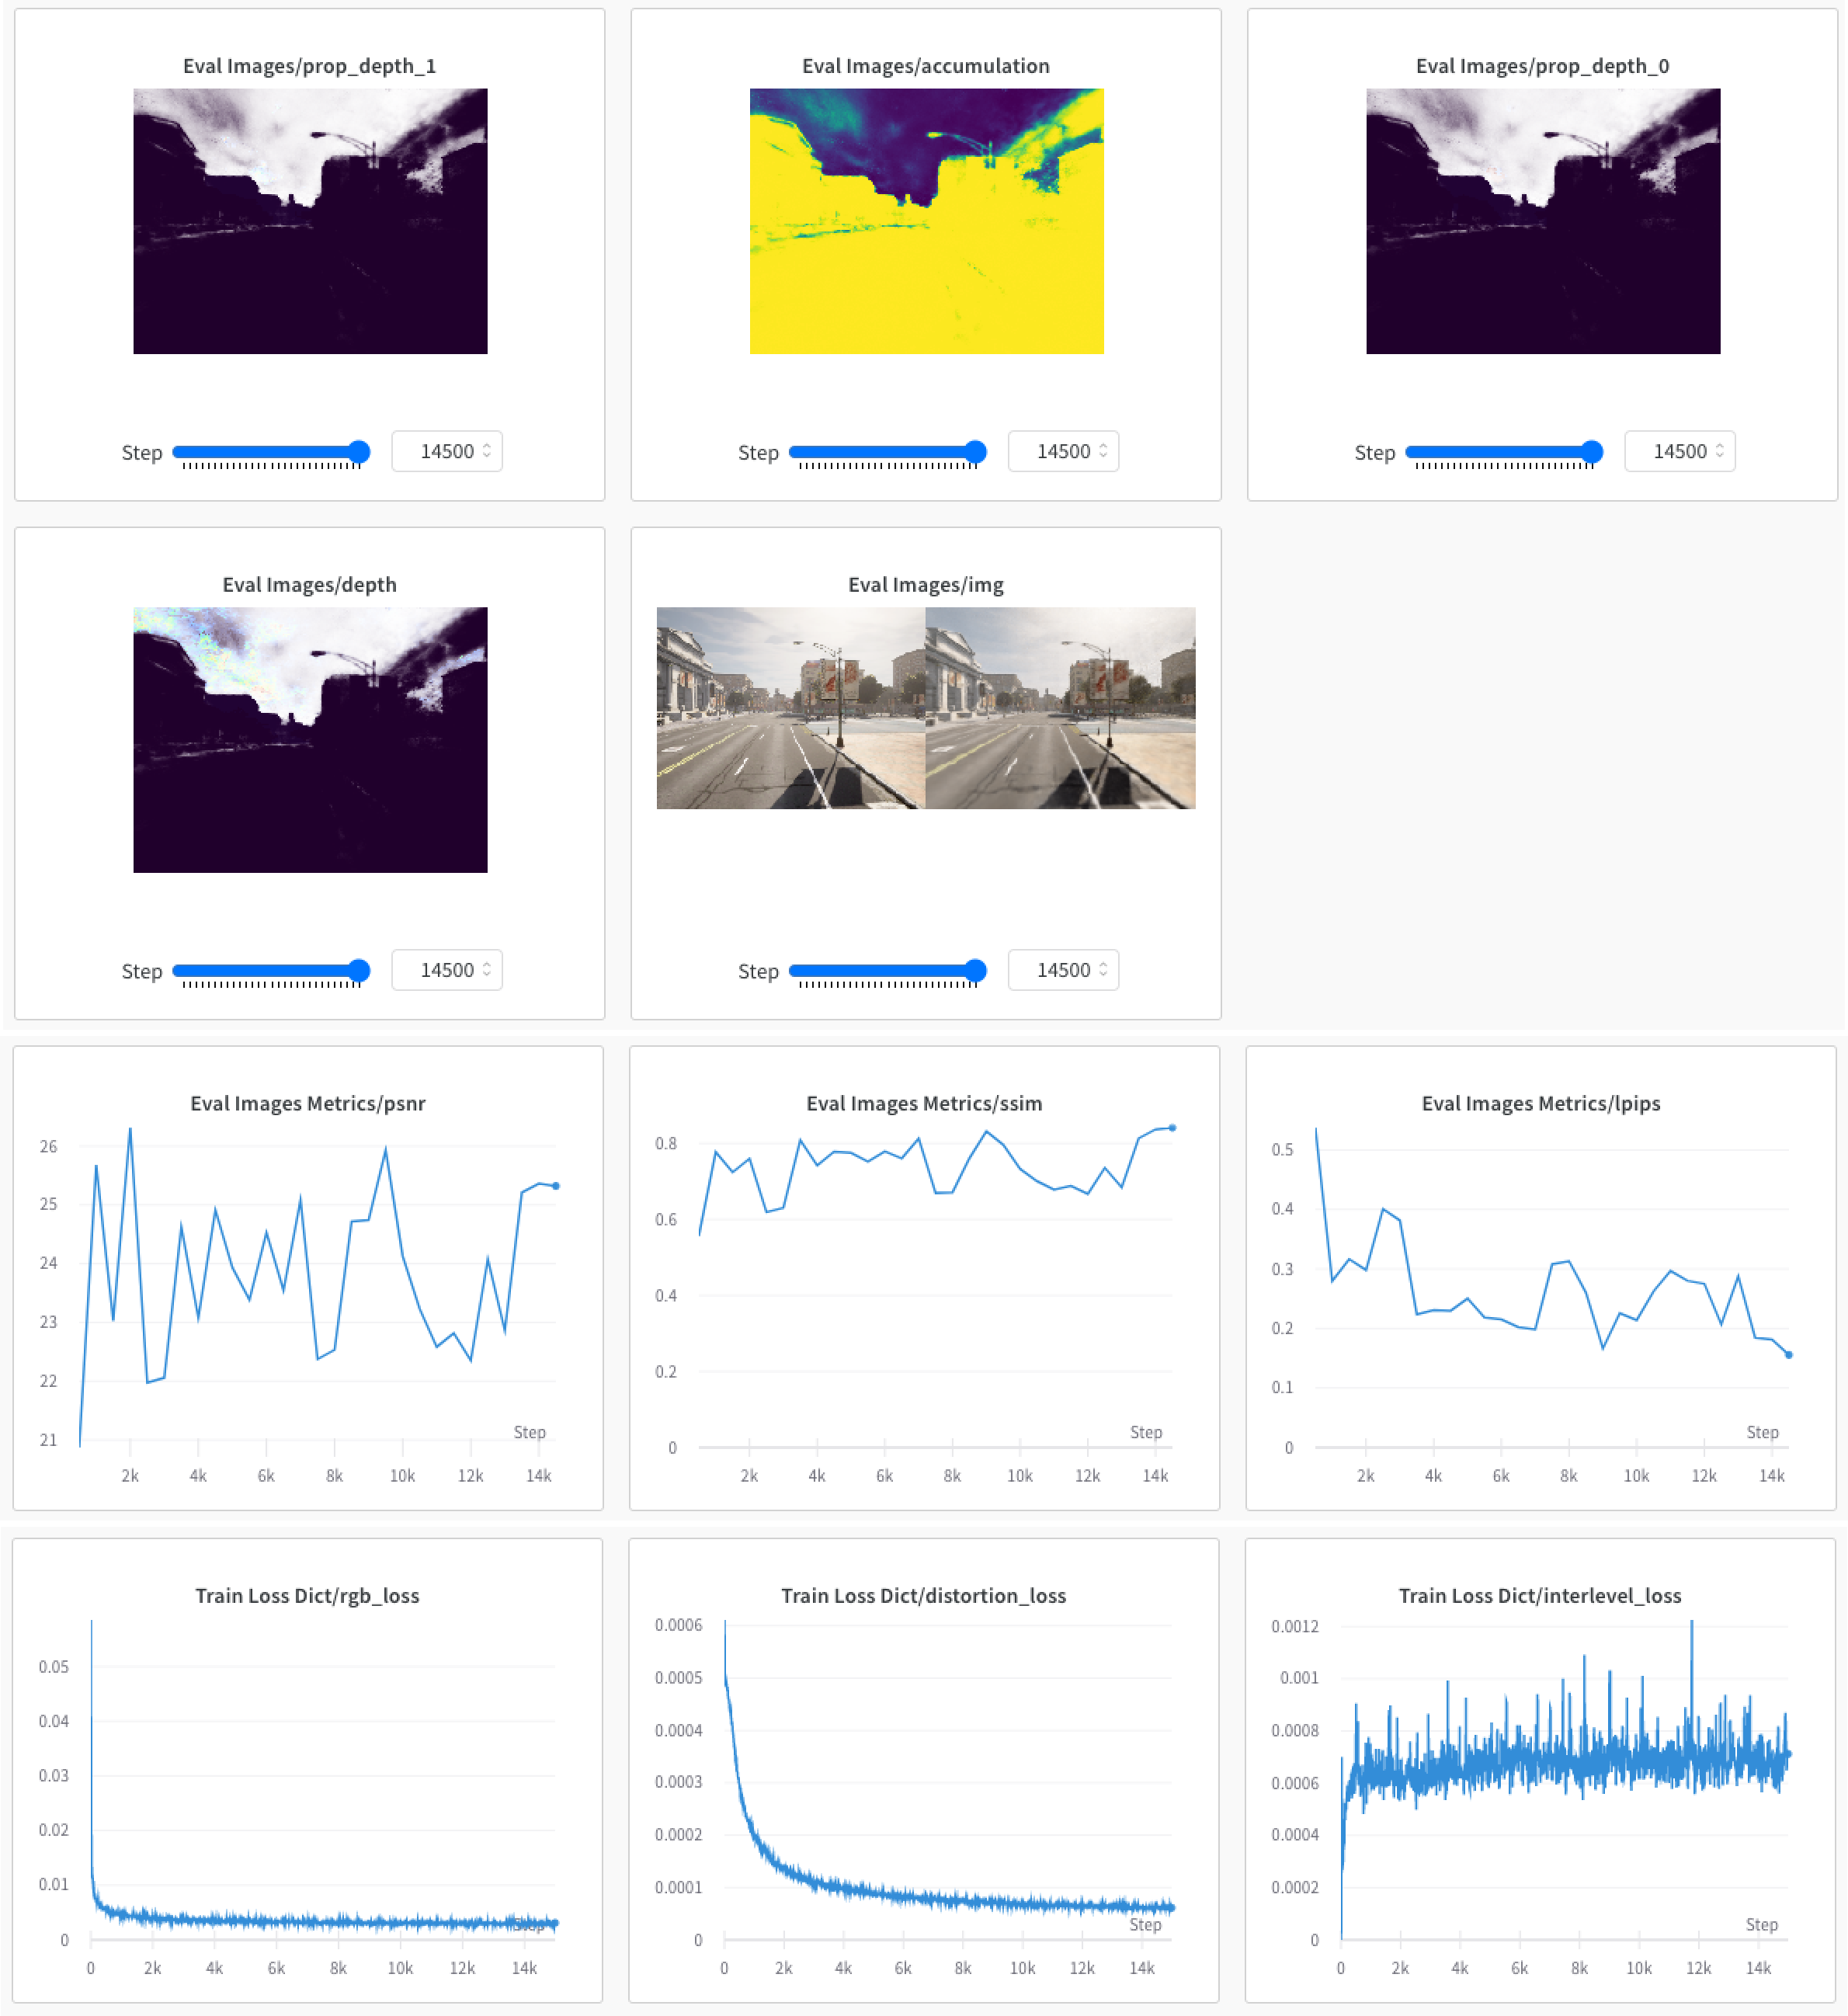
\includegraphics[width=1.0\textwidth]{figures/wandb-eval-data.png}
    \caption{Selection of evaluation data from Weights \& Biases \cite{wandb} for a NeRF training on a segment of synthetic data from CARLA.}
    \label{fig:wandb-eval-data}
\end{figure}

\subsubsection{Render}
%However, comparing experiments across different models and datasets with custom camera paths that will be slightly different for run/scene can be time-consuming and challenging. To address this issue, a script was developed to extract the ground truth camera path and use it in conjunction with the input images and trained NeRF model to create a side-by-side rendering. This approach has proven to be a useful means of qualitatively evaluating the performance of the NeRF models.

Although the quantitative metrics offer valuable insights into the quality of the model, it is crucial to assess the qualitative output. Consequently, all trained NeRF models are rendered in order to visually compare the results across different methods, configurations, and datasets.

The Nerfstudio API provides a script for rendering trained NeRF models given a camera path; a sequence of camera poses, each with a corresponding field of view and aspect ratio. The Nerfstudio viewer, depicted in \autoref{fig:nerfstudio-viewer-overview}, enables the creation and editing of camera paths, which can be exported and used for rendering. In addition to the possibility to create a custom camera path, a script to render the NeRF based on the input data's camera path was created. This option enables the creation of a side-by-side render, a useful and intuitive way to evaluate how well the NeRF has learned the input scene, i.e. qualitatively assessing the NeRF's performance.

\begin{figure}[H]
    \centering
    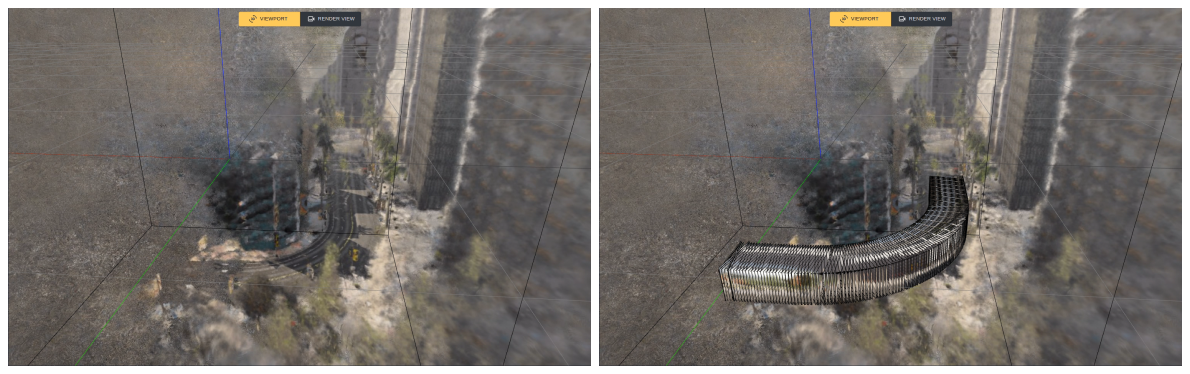
\includegraphics[width=1.0\textwidth]{figures/nerfstudio-viewer-overview.png}
    \caption{An overview of the Nerfstudio viewer. The scene seen on the left has been trained on the set of images and camera poses revealed in the image to the right.}
    \label{fig:nerfstudio-viewer-overview}
\end{figure}
%\begin{figure}[ht]
\centering
\begin{lstlisting}[language=json,linewidth=0.9\linewidth]
{
  "camera_type": "perspective",
  "render_height": 1080,
  "render_width": 1920,
  "fps": 24,
  "seconds": 10,
  "smoothness_value": 0.4624,
  "is_cycle": true,
  "camera_path": [
    {
      "camera_to_world": [
          0.0387,  0.0484,  0.9980,  0.4483,
          0.9992, -0.0018, -0.0386,  0.9853,
         -2.0166,  0.9988, -0.0485, -0.0018,
          0,       0,       0,       1
      ],
      "fov": 90,
      "aspect": 1.6678200692041523
    },
    ...
  ],
  "keyframes": [...],
}

\end{lstlisting}
\caption{Example of a \textit{camera-path.json}-file used to render a specific path for a trained NeRF in the Nerfstudio API.}
\label{code:camera-path-example}
\end{figure}




\begin{comment}
% TODO: If I'm to use this, I have to double check if it's correct
\begin{equation} \label{eq:distortion_loss}
\mathcal{L}_{\text{distortion}} = \frac{1}{N} \sum_{i=1}^{N} \left(\sum_{j=1}^{M_i} w_{ij} \sum_{k=1}^{M_i} w_{ik} \left| \frac{t_{ij} + t_{ik}}{2} - \frac{t_{i,j-1} + t_{i,k-1}}{2} \right| \right) + \frac{1}{3N} \sum_{i=1}^{N} \sum_{j=1}^{M_i} w_{ij}^2 (t_{ij} - t_{i,j-1})
\end{equation}

\begin{center}
    \small{where $N$ is the number of ray samples, $M_i$ is the number of samples for the $i$-th ray, $w_{ij}$ is the weight for the $j$-th sample of the $i$-th ray, $t_{ij}$ is the $j$-th sample of the $i$-th ray in the $s$-domain, and $t_{i,j-1}$ is the $(j-1)$-th sample of the $i$-th ray in the $s$-domain.}
\end{center}


\begin{equation} \label{eq:interlevel_loss}
\mathcal{L}_{\text{interlevel}} = \frac{1}{N} \sum_{i=1}^{N-1} \frac{1}{M_i} \sum_{j=1}^{M_i} \left(\max(0, w_j - w_{\text{outer},ij})\right)^2 \cdot \frac{1}{w_j + \epsilon}
\end{equation}

\begin{center}
    \small{where $N$ is the number of ray samples, $M_i$ is the number of samples for the $i$-th ray, $w_j$ is the weight for the $j$-th sample of the $i$-th ray, $w_{\text{outer},ij}$ is the upper bound of the inner histogram for the $j$-th sample of the $i$-th ray, and $\epsilon$ is a small constant.}
\end{center}
\end{comment}




%\section{Establish a CARLA-baseline}
\section{Establishing the CARLA-Baseline}
\begin{comment}
Premise: Have a pipeline to test multiple CARLA-setups
Question: How do I find a CARLA-baseline?

\begin{itemize}
    \item Why do I need a baseline?
    \item How do I find suitable experiments?
    \item How do I evaluate the experiments against each other?
\end{itemize}
\end{comment}

A pipeline to evaluate numerous CARLA configurations to identify a configuration that generates high-quality data for NeRF training has been established. In order to facilitate further experiments, a baseline need to be created.

The experiments chosen to define a suitable baseline are mostly based on heuristics and knowledge of what's important for good NeRF results. When capturing video or images for a NeRF it’s important that the scene is well-lit, that you capture non-blurry images, and that there are no transient objects present. If the camera poses of the images you capture are to be approximated with the use of SfM-methods like COLMAP, it's also very important that the images have an overlap in order to secure feature-matching across the images. The five experiments chosen to define the baseline, which will be elaborated upon in \autoref{sec:experiments-and-results}, were:

\begin{itemize}
    \item \textbf{Camera setup:} How many cameras should be mounted to the ego vehicle, and in what translation and rotation?
    \item \textbf{Capacity:} How long should the segments used to capture data be?
    \item \textbf{Number of frames:} How many frames to capture?
    \item \textbf{Image size:} What resolution should the mounted cameras capture at?
    \item \textbf{Vehicle speed:} At what speed should the ego vehicle drive while capturing data?
\end{itemize}

The best results from each of the experiments, based on qualitative results and quantitative metrics discussed in \autoref{sec:evaluating-nerfs}, were used to iteratively build a baseline used for further experiments.
















%\section{Use the CARLA-baseline}
\section{Comparative Experiments with the CARLA-Baseline}
\begin{comment}
Premise: Have a CARLA-baseline for further experiments
Question: Which further experiments should I conduct?

\begin{itemize}
    \item Find the efficiency of pose refinement
\end{itemize}
\end{comment}

With a defined baseline, we can now evaluate the impact of different NeRF- and capture settings on the quality of the resulting models. This provides a starting point for conducting further experiments, which can be systematically varied to explore the factors that impact the quality of resulting trained NeRF. Additionally, we can simulate real-world capture scenarios using the synthetic data generated by the baseline. The specific experiments ran with the baseline, elaborated upon in \autoref{sec:experiments-and-results}, were:

\begin{itemize}
    \item \textbf{Noisy sensor readings:} Noise in the camera pose due to inaccurate readings from the GPS/GNSS.
    \item \textbf{Approximated poses vs. perfect poses:} How effective is COLMAP in approximating the camera poses, as opposed to the perfect camera poses extracted from CARLA?
    \item \textbf{Different models:} How do the different NeRF models perform against each other?
    \item \textbf{Improve capacity - Block NeRF PoC}: How can we train NeRFs on increasingly larger scenes?
\end{itemize}




















































%\section{Extend the CARLA-baseline to support large scale scenes} \label{sec:method-block-nerf}
\section{Extending the Pipeline to Support Large-Scale Scenes} \label{sec:method-block-nerf}

\begin{comment}
Premise: Have found the CARLA-baseline to work well on shorter segments. As discussed multiple papers, the capacity is limited.
Premise \#2: Since I operate in a synthetic environment, I have perfect poses which simplifies the process.
Question: How do I implement Block-NeRF in Nerfstudio, given perfect poses?

\begin{itemize}
    \item Split the dataset into multiple datasets
    \item Train each seperately
    \item Create a camera path
    \item Render the camera path for each NeRF
\end{itemize}
\end{comment}

The NeRF model in the defined baseline has proven to perform well. When we change the route of the CARLA-baseline and create a larger dataset, spanning kilometers of road data, the NeRF models evidently have a hard time generating high-quality image synthesis. That result is expected as the models' underlying MLPs only have a certain capacity. We could increase the capacity by increasing the number of hidden layers and neurons per layer, but this would lead to linearly increasing training -and rendering times. Rendering is already an expensive operation which further supports the claim for another solution.

As discussed in \autoref{sec:block-nerf} it is an open research field within the NeRF community to expand the capability of NeRFs to enable the representation of large scenes. Compared to the other fields covered in NeRF research, there aren't a lot of papers exploring large-scale NeRFs, which might be due to the amount of data needed and the corresponding data capture endeavor. Luckily, we have constructed a pipeline that automates synthetic data capture and the subsequent processing, training, evaluation and rendering of the NeRF. Due to this we expand the pipeline to enable the evaluation of a large-scale NeRF approach, based on a naive implementation of Block-NeRf \cite{tancik_block-nerf_2022}.

% Explain the naive Block NeRF implementation
One of the main challenges in implementing Block-NeRF is obtaining the camera poses for the captured images. Traditional SfM methods, such as COLMAP, become computationally expensive and slow when dealing with large datasets, as is demonstrated by the feature matching complexity overview presented in Table \ref{tab:colmap-feature-complexity}. However, being in possession of the image's corresponding camera poses simplifies the process. Assuming we have both, the steps for creating a Block-NeRF model can be summarized as follows:

\begin{itemize}
    \item \textbf{Split the dataset into multiple smaller datasets:} 

    The \textit{split\_transforms} function takes an original \texttt{transforms.json} file and a sequence of images and splits them into $n$ roughly equal-sized new datasets, which are formatted according to the structure shown in \autoref{fig:nerfstudio-file-structure}, resulting in a file structure shown in \autoref{fig:block-nerf-file-structure}.

    \item \textbf{Train separate NeRFs on the split dataset:} 

    Run a standard training loop on each of the $n$ datasets created in the previous step.
    
    \item \textbf{Create a camera path spanning the segments contained in the complete dataset:}
    
    There are multiple options for creating the camera path: The camera path can be created in the Nerfstudio viewer, you could leverage a previously exported camera path, or you could use a helper function to leverage the camera path of the input images which will later also be used to generate the side-by-side render. No matter which option you choose, an important aspect in this naive implementation is that the camera-to-world matrices in the camera path are in the same scale and coordinate system as the Block-NeRF's \texttt{transforms.json}-files.
    
    \item \textbf{Create a lookup table for which Block to render which camera pose:}

    In order to know which NeRF to render given a specific 3D point and direction, expressed by the $4x4$ camera-to-world matrix in the camera path, we create a naive lookup table. The lookup table is indexed on the camera path's location index and returns the Block-NeRF with the minimum Euclidean distance.

    \item \textbf{Modify the camera path to account for the offset, transformations, and scales of each NeRF:}
    
    Before a NeRF is trained, the input camera poses are scaled to fit a $[-1, 1]$ bounding box, and transformed so that the average up vector is aligned with the Z-axis. The respective transformation which is carried out to make the training easier is stored in a \texttt{dataparser\_transforms.json}-file containing the applied transform matrix and scale. Each of the Block-NeRF's \texttt{dataparser\_transforms.json}-file is different, and in order to render the desired camera path seamlessly across the different NeRFs according to the lookup table, we have to augment it to account for the transformations. We achieve this by creating a new, transformed camera path where the segments which are to be rendered by $\text{Block-NeRF}_i$ have their camera-to-world transformed by applying $\text{Block-NeRF}_i$'s scale $s$ and transformation matrix $t$. 
    
    \item \textbf{Render the created camera path:}

    Building upon Nerfstudio's render script, the lookup table is passed as a parameter and used to conditionally choose which model to render. As all the changes to the camera path have been done a priori, the resulting render is a seamless video through the scene leveraging multiple Block-NeRFs.
\end{itemize}



\begin{comment}
\begin{algorithmic}[1]
\Function{transform\_to\_single\_camera\_path}{}
    \State $block\_lookup$ \Comment{Lookup block to render at a certain c2w}
    \For{$c2w$ \textbf{in} $camera\_path$}
        \State $block \gets block\_lookup[c2w]$
        \State $t \gets block.dataparser\_transform["transform"]$
        \State $s \gets block.dataparser\_transform["scale"]$
        \State $new\_c2w \gets (t \times c2w) \times s$
        \State $camera \gets new\_c2w$
    \EndFor
\EndFunction
\end{algorithmic}


% TODO: If I'm to use this algorithm I have to go over it and fix it.
\begin{algorithmic}[1]
\Function{transform\_to\_single\_camera\_path}{$camera\_path\_path, block\_lookup, dataparser\_transform\_paths, export\_dir$}
    \State $original\_camera\_path \gets$ \Call{load\_json}{$camera\_path\_path$}
    \State $new\_camera\_path \gets$ \Call{copy.deepcopy}{$original\_camera\_path$}

    \For{$i \gets 0$ \textbf{to} $len(new\_camera\_path["camera\_path"]) - 1$}
        \State $block\_name \gets block\_lookup[str(i)]$
        \State $transform \gets$ \Call{load\_json}{$dataparser\_transform\_paths[block\_name]$}
        \State $t \gets$ \Call{np.array}{$transform["transform"]$}
        \State $s \gets transform["scale"]$

        \State $c2w \gets$ \Call{np.array}{$new\_camera\_path["camera\_path"][i]["camera\_to\_world"]$}.\Call{reshape}{4, 4}
        \State $c2w \gets (t \times c2w) \times s$
        \State $c2w \gets$ \Call{np.vstack}{($c2w$, \Call{np.array}{[0, 0, 0, 1]})}
        \State $new\_camera\_path["camera\_path"][i]["camera\_to\_world"] \gets c2w.\Call{reshape}{16}.\Call{tolist}{}$
    \EndFor
\EndFunction
\end{algorithmic}
\end{comment}

\begin{figure}[ht]
\centering
\begin{forest}
for tree={
      parent anchor=south west,
      child anchor=west,
      anchor=mid west,
      inner ysep=1pt,
      grow'=0,
      align=left,
      edge path={
        \noexpand\path [draw, \forestoption{edge}] (!u.parent anchor) ++(1em,0) |- (.child anchor)\forestoption{edge label};
      },
      font=\sffamily,
      if n children=0{}{
        delay={
          prepend={[,phantom, calign with current]}
        }
      },
      fit=band,
      before computing xy={
        l=2em
      }
    }
[block\_nerf\/
[ block\_0\/
  [ images/
    [ 0001.png ]
    [ 0002.png ]
    [ 0003.png ]
    [ \ldots{} ]
  ]
  [ transforms.json ]
]
[\ldots{}]
[ block\_n\/
  [ \ldots{} ]
]
]
\end{forest}
\caption[Block-NeRF file structure]{Block-NeRF file structure after having split a single dataset into multiple smaller datasets.}
\label{fig:block-nerf-file-structure}
\end{figure}

%A large part of what is tricky with implementing Block-NeRF is obtaining the captured images' camera poses. COLMAP becomes painfully slow with large datasets, as can be seen by the feature matching complexity overview in \autoref{tab:colmap-feature-complexity}. When you capture the images' corresponding camera pose simultaneously as you capture the image, it's another story. With both the images and camera poses, the main steps in creating the Block NeRF are 1) splitting the dataset into multiple smaller datasets, 2) training separate NeRFs on the split datasets, 3) creating a camera path and modifying it to take into account the offset between each NeRF, 4) and lastly rendering the camera path by combining renders from suitable NeRFs.














%\section{Extending the pipeline to enable input of real data} \label{sec:extending-real-data}
\section{Extending the Pipeline to Support Real Data} \label{sec:extending-real-data}

\begin{comment}
Premise: Have a working pipeline to collect, train and render novel views from CARLA
Question: How can this pipeline be extended to enable input of real data?

\begin{itemize}
    \item How to collect images and camera poses from the car?
    \item Which changes had to be done to the pipeline to support this change?
\end{itemize}
\end{comment}

%\begin{figure}[!h]
    \centering
    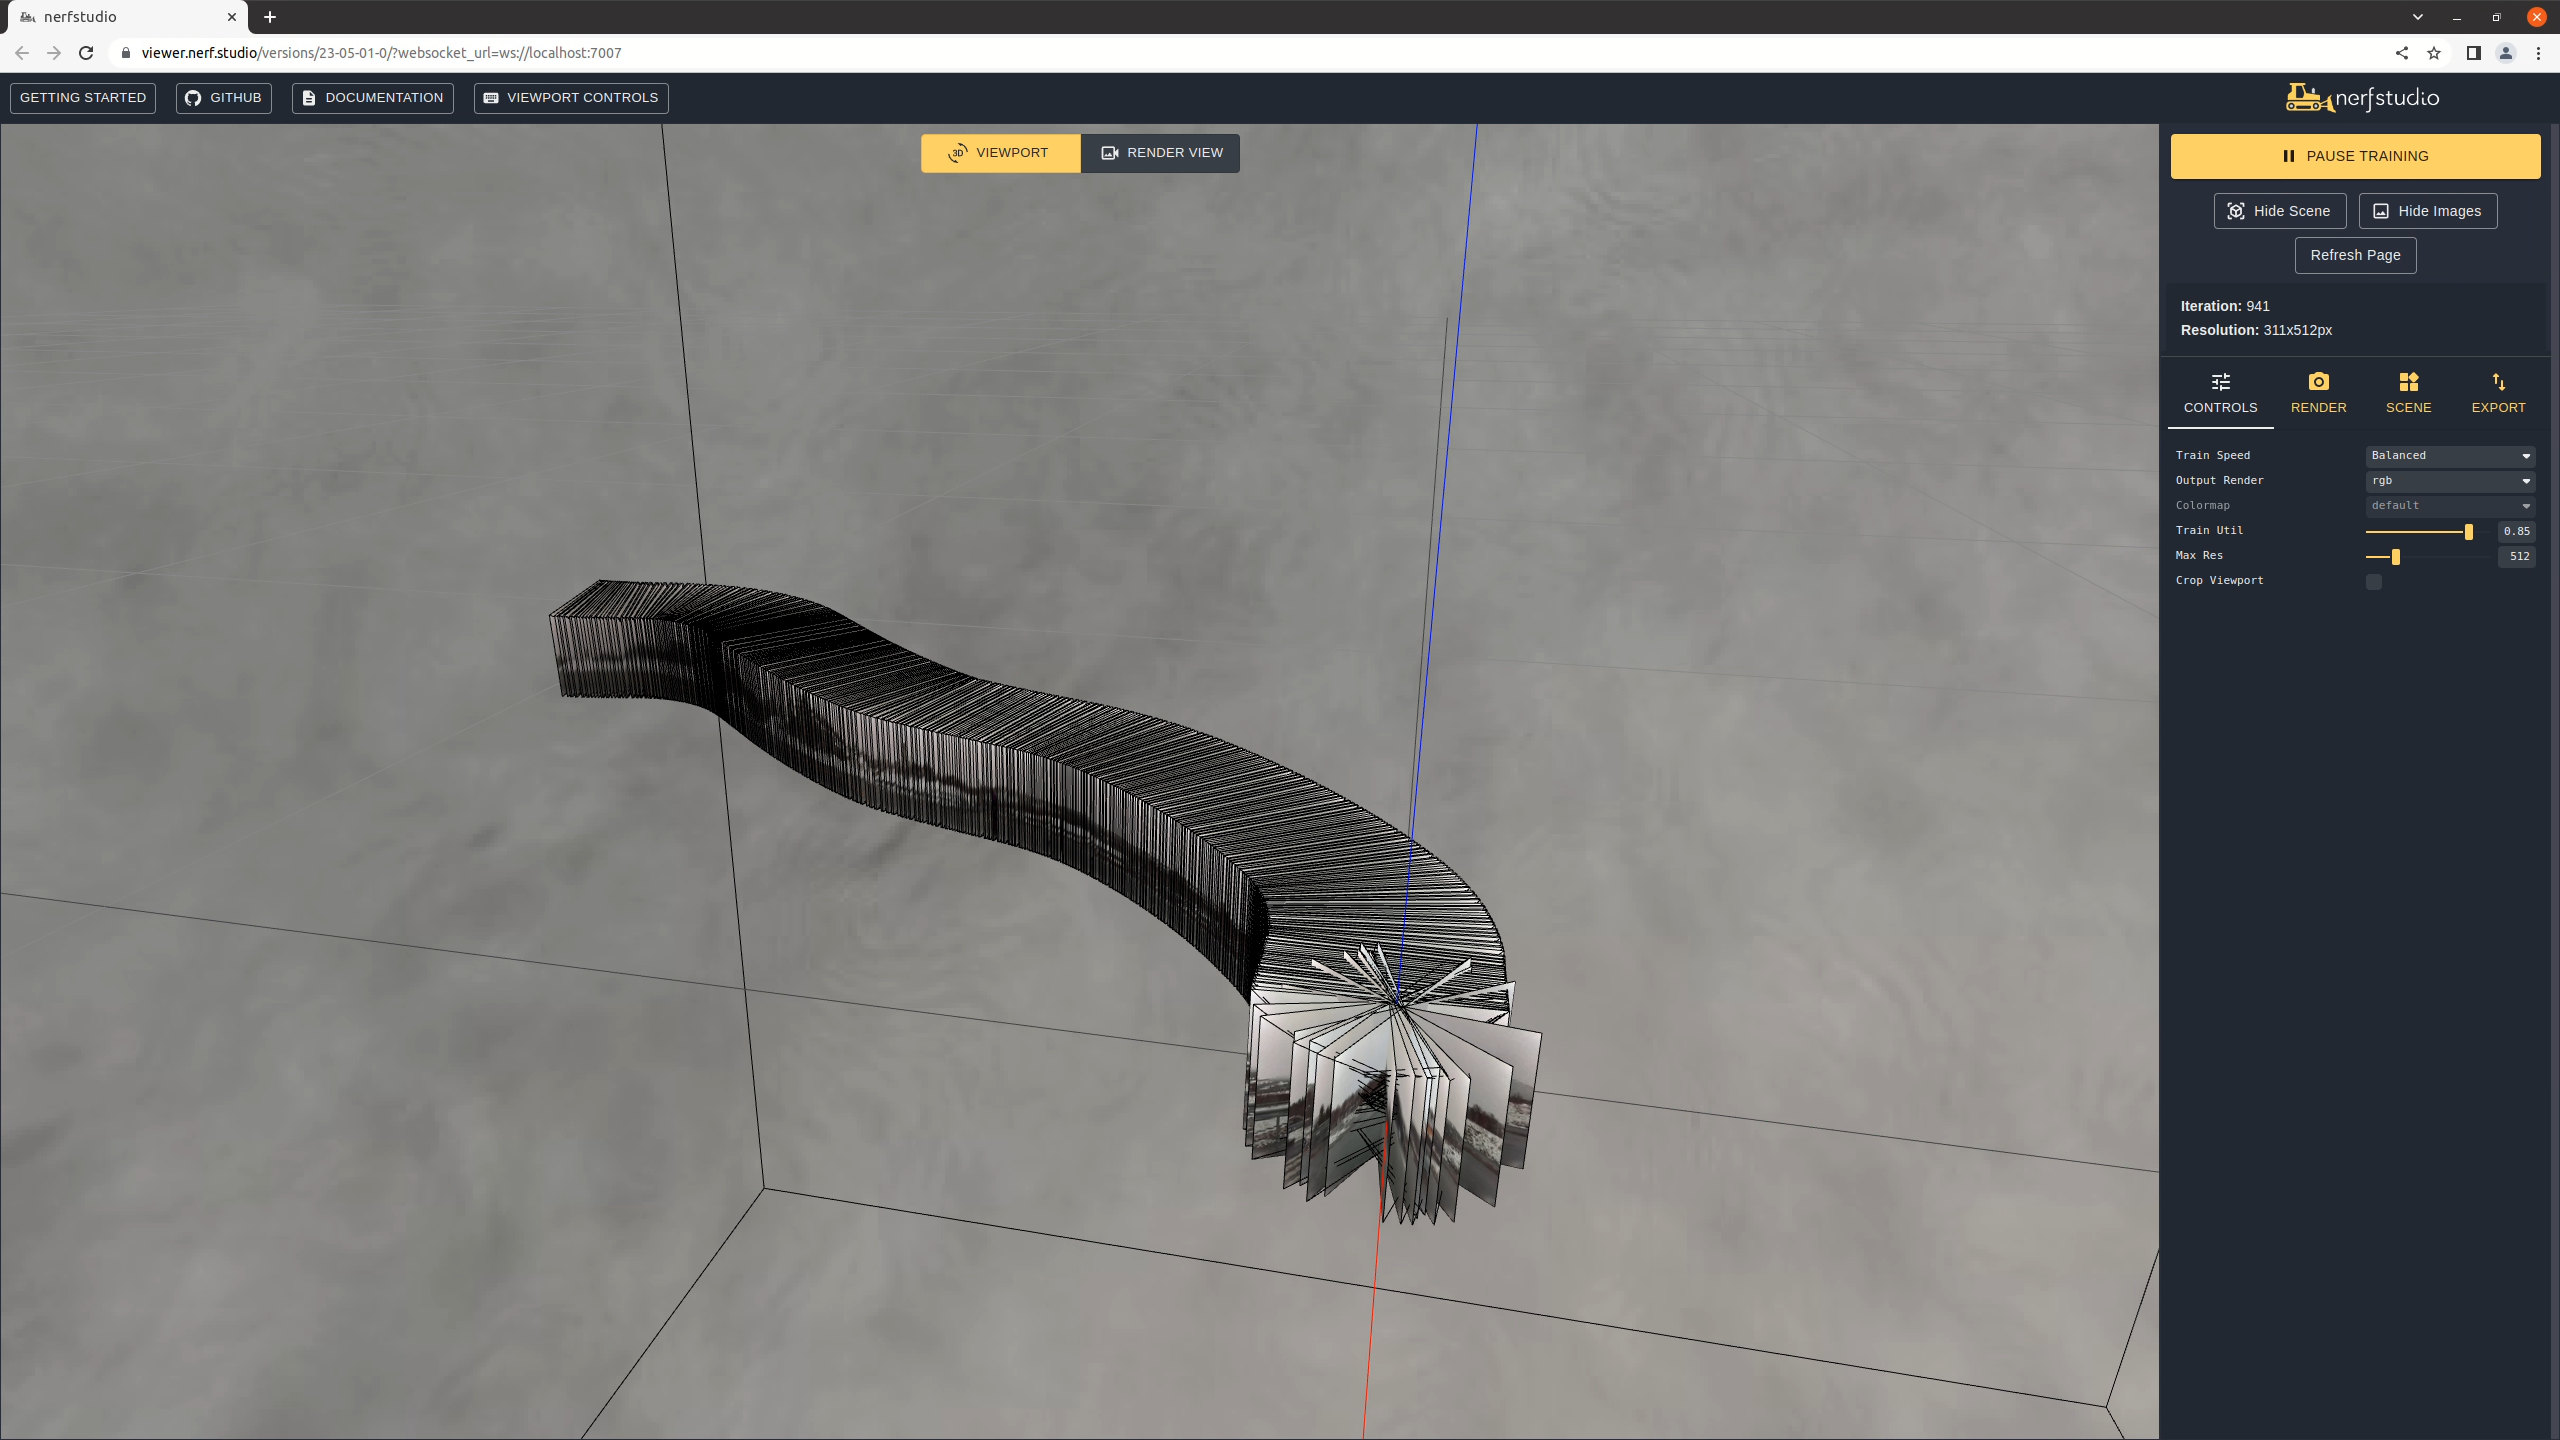
\includegraphics[width=1.0\textwidth]{figures/nerfstudio_real_data_estimated_poses.png}
    \caption{Real data with estimated poses viewed in the Nerfstudio Viewer}
    \label{fig:nerfstudio_real_data_estimated_poses}
\end{figure}

\begin{comment}
Introduction
- Making NeRFs with real data is the usual way to go about generating NeRFs.
- The challenge is in capturing this data from cameras mounted on vehicles, in uncontrolled environment.

How do I expand the pipeline?
- How is the data captured? Introduce the NAPLab-car, the sensors, etc.
- How do I read this data? Mention the Aksel and Mathias' repository.
    - Use FFMPEG to read the .h264-video and serve the frames with a generator-function.
    - Use regex to parse a file with GPS data formatted as NMEA (National Marine Electronics Association) sentences, a standard messages used by GPS (Global Positioning System) receivers to communicate with other devices, such as computers or chartplotters. Each GPS-datapoint is seved with a generator-function the same way as with the video-frames.
    - The camera is synchronized to the closest frame in time to the GPS timestamp using custom code. "- Custom code is used to synchronize the camera to the frame closest in time with the GPS timestamp."
    - After synchronization, I can loop through the synchronized sensor data with a regular loop.
- Premise: Have synchronized image- and GPS-data.
- Create a NAPLabDataParser that implements the same methods as the CarlaDataParser. The main difference is in the implementation of the transform-function. 
- The transformation matrix is created by :
    - Store the initial GPS lat, long and alt, and use it as the reference point.
    - The reference point is utilized in order to convert latitude, longitude, altitude of subsequent GPS-readings to North, East, Down from the observer, i.e. the reference point.
    - NED is then converted to ENU and then to blender coordinate conventions.
    - The rotation is estimated with trigonometry by comparing subsequent GPS-readings.
    - The translation and rotation is combined into a transformation matrix.
- The intrinsics are computed in the same way as discussed in \autoref{sec:carla-to-nerfstudio}.
- The transformation matrix and intrinsics are combined into a transform.json
- The exported transform.json and images are in the same format as the output from the CarlaDataParser, so the following pipeline remains unchanged.
\end{comment}

The pipeline from data capture in CARLA to image synthesis with a trained NeRF has demonstrated efficacy. This final section of the method-chapter discusses how the pipeline is extended to enable the input of real data, not captured in a virtual environment like the CARLA simulator.

The traditional approach for generating NeRFs involves the use of real data. The real data is usually captured from handheld cameras. With handheld cameras it is uncomplicated to capture well-lit, non-blurry, object-centric images that doesn't contain transient objects. Until now we've used a virtual environment to capture data as it provides a fully controllable environment in which we can test different setups and ensure optimal conditions. The following challenge in this project is capturing high-quality data from sensors, mounted to a moving vehicle, that is suitable for training NeRF models.

To capture data, we utilized the\acrshort{naplab} car \cite{naplab}. The NAPLab car is fitted with multiple sensors, including cameras, Global Positioning System (GPS)/Global Navigation Satellite System (GNSS), and Lidar. The cameras capture data with a resolution of $1920 \times 1080$. The GPS/GNSS-system consists of two Swift Navigation Duro Ruggedized Receivers \cite{swift_navigation_duro_manual}, which offer superior positioning accuracy compared to regular GPS/GNSS systems. According to the manufacturer’s documentation, each Duro module has a horizontal position accuracy of 0.75 meters (Circular error probability [CEP] of 50 in Satellite-Based Augmentation System [SBAS] mode) without Real-time kinematic positioning (RTK), and can achieve centimeter-level accuracy with RTK enabled. This high level of accuracy enables the capture of rough camera poses alongside the images.

After having captured data with the NAPLab car, the data has to be parsed and processed before it can be transformed into the expected Nerfstudio-format. A repository\footnote{\url{https://github.com/aasewold/experiments/}} that streamlines the reading and parsing of NAPLab's data into a manageable format was leveraged. In order to read the video data, FFMPEG is utilized to transform .h264-files into sequences of \texttt{np.ndarray}s that are subsequently served by a generator function. The GPS data is formatted as National Marine Electronics Association (NMEA) sentences, a message standard used by GPS receivers to communicate with other devices. This GPS data is read and parsed using regex and subsequently served by a generator function. 

A key aspect of the data parsing is the synchronization of the camera with the GPS timestamp. This is achieved by leveraging functionality from the same repository that aligns the camera with the frame closest in time to the GPS timestamp. Following synchronization, the sensor data can be accessed and further processed using a regular loop.

The synchronized data have to be converted into Nerfstudio's data format in order to be used in the predefined pipeline. In order to achieve this, a \texttt{NAPLabDataParser} that implements the same methods as the \texttt{CarlaDataParser}, is created. The primary difference is the implementation of the transformation function that converts the translation and rotation data from one coordinate convention to another. The transformation matrix construction process involves several steps:

\begin{itemize}
    \item The initial GPS latitude, longitude, and altitude readings are stored as the reference point.
    \item The \texttt{geodetic2ned} function from the \texttt{pymap3d} library \cite{Hirsch_PyGemini} is used to transform GPS data into North, East, Down (NED) coordinates.
    \item The NED coordinates are then converted to East, North, Up (ENU) coordinates and then to Blender coordinate conventions.
    \item The cameras' rotation is estimated by comparing adjacent GPS data points using trigonometry.
    \item The resulting translation and rotation data are combined into a single transformation matrix.
\end{itemize}

The computation of intrinsic values follows the same methodology as discussed in \autoref{sec:carla-to-nerfstudio}. These intrinsics, in combination with the transformation matrix, are assembled into a \texttt{transforms.json} file. The output from the \texttt{NAPLabDataParser}, i.e., the \texttt{transforms.json} file and images, is in the same format as that from the \texttt{CarlaDataParser}. Therefore, the subsequent stages of the pipeline remain unaffected, ensuring the smooth extension from synthetic to real data inputs.

The dataset captured from the NAPLab car is presented in \autoref{fig:naplab-dataset}.

\begin{figure}[h]
    \centering
    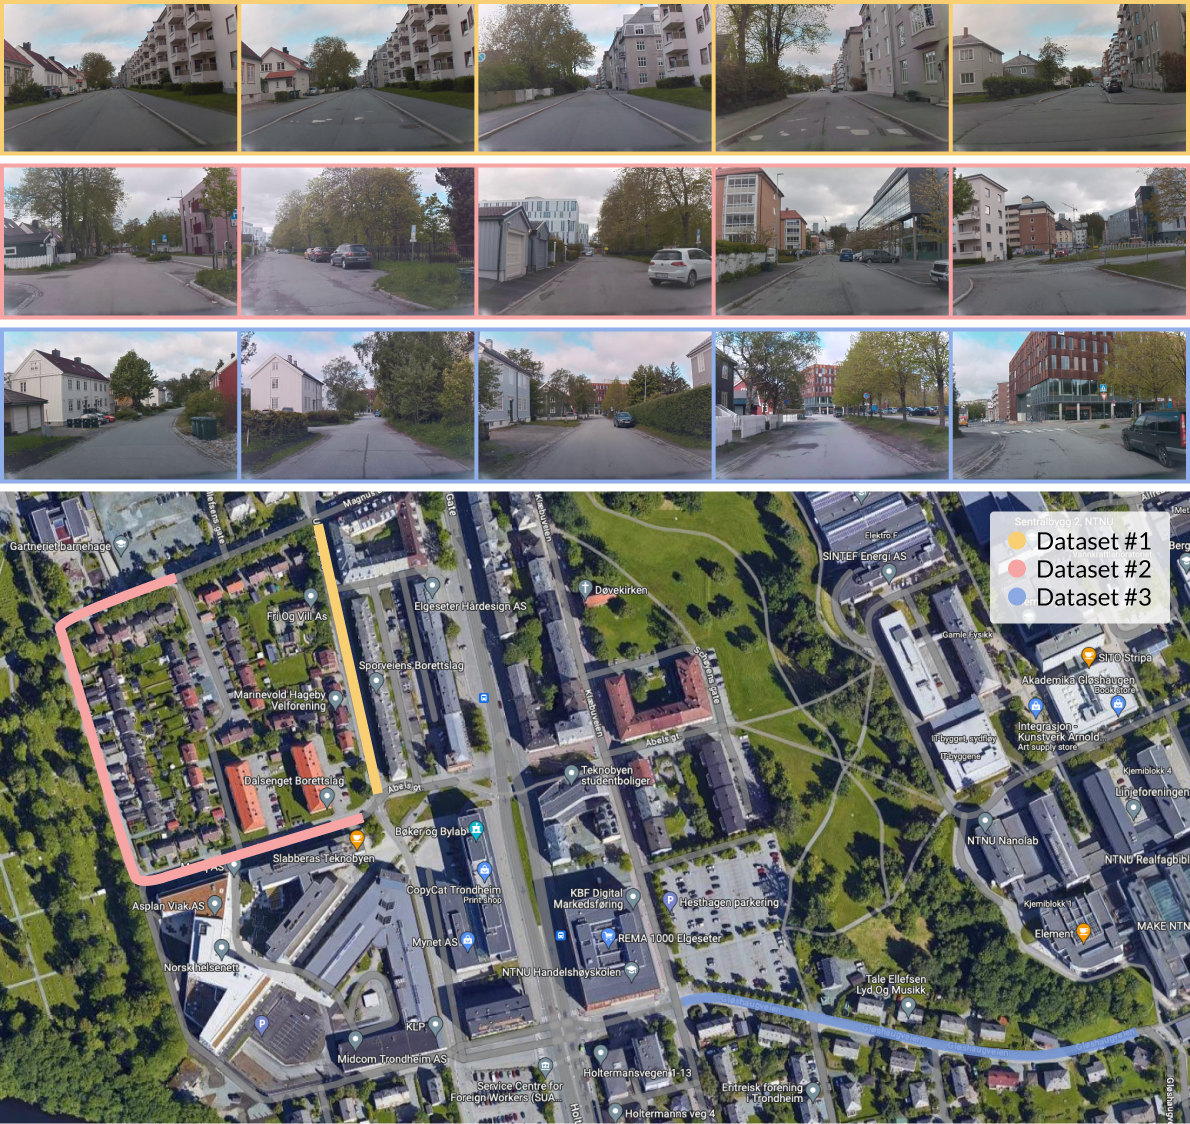
\includegraphics[width=1.0\textwidth]{figures/naplab-dataset.png}
    \caption[The datasets captured from the NAPLab car.]{Overview of the datasets of real data captured from the NAPLab car. 1) contains 235 images over a straight road segment of approximately 170m, 2) contains 199 images over a segment of approximately 380m, 3) contains 160 images over a segment of approximately 280m.}
    \label{fig:naplab-dataset}
\end{figure}





\begin{comment}
The traditional approach for generating Neural Radiance Fields (NeRFs) involves the use of real data. However, collecting this real data presents a unique challenge when dealing with cameras mounted on vehicles operating in uncontrolled environments. Overcoming this obstacle requires an innovative expansion of the existing data processing pipeline.

Data capture is achieved with the assistance of a specially outfitted vehicle, known as the NAPLab-car, equipped with an array of sensors for comprehensive environmental data collection. Subsequently, the captured data is read and processed using the repository developed by Aksel and Mathias.

This repository utilizes FFMPEG software to read the .h264-video, serving the video frames through a generator function. In parallel, a regular expression (regex) is used to parse GPS data structured as NMEA (National Marine Electronics Association) sentences - standard messages exchanged between GPS receivers and auxiliary devices like computers or chartplotters. Each parsed GPS datapoint is then served via a generator function akin to the video frames.

A key aspect of the pipeline expansion is the synchronization of the camera with the GPS timestamp. This is achieved with custom code that aligns the camera with the frame closest in time to the GPS timestamp. Following synchronization, the sensor data can be accessed and navigated using a regular loop.

Building on this premise of synchronized image and GPS data, a NAPLabDataParser is created to mimic the functionality of the CarlaDataParser. The primary distinction lies in the implementation of the transform function. The transformation matrix construction process involves several steps:

- The initial GPS latitude, longitude, and altitude readings are stored and utilized as a reference point.
- This reference point serves as a basis to convert subsequent GPS readings into North, East, Down (NED) coordinates relative to the observer.
- NED coordinates are subsequently converted to East, North, Up (ENU) and further to Blender coordinate conventions.
- Subsequent GPS readings are compared to estimate rotation using trigonometry.
- Finally, the translation and rotation data are integrated into a single transformation matrix.

The computation of intrinsic values follows the same methodology as discussed in \autoref{sec:carla-to-nerfstudio}. These intrinsics, in combination with the transformation matrix, are assembled into a transforms.json file.

The output from the NAPLabDataParser, i.e., the transforms.json file and images, is analogous in format to that from the CarlaDataParser. Therefore, the subsequent stages of the pipeline remain unaffected, ensuring the smooth transition from synthetic to real data inputs.
\end{comment}